\documentclass[10pt]{beamer}\usepackage[]{graphicx}\usepackage[]{color}
%% maxwidth is the original width if it is less than linewidth
%% otherwise use linewidth (to make sure the graphics do not exceed the margin)
\makeatletter
\def\maxwidth{ %
  \ifdim\Gin@nat@width>\linewidth
    \linewidth
  \else
    \Gin@nat@width
  \fi
}
\makeatother

\definecolor{fgcolor}{rgb}{0.345, 0.345, 0.345}
\newcommand{\hlnum}[1]{\textcolor[rgb]{0.686,0.059,0.569}{#1}}%
\newcommand{\hlstr}[1]{\textcolor[rgb]{0.192,0.494,0.8}{#1}}%
\newcommand{\hlcom}[1]{\textcolor[rgb]{0.678,0.584,0.686}{\textit{#1}}}%
\newcommand{\hlopt}[1]{\textcolor[rgb]{0,0,0}{#1}}%
\newcommand{\hlstd}[1]{\textcolor[rgb]{0.345,0.345,0.345}{#1}}%
\newcommand{\hlkwa}[1]{\textcolor[rgb]{0.161,0.373,0.58}{\textbf{#1}}}%
\newcommand{\hlkwb}[1]{\textcolor[rgb]{0.69,0.353,0.396}{#1}}%
\newcommand{\hlkwc}[1]{\textcolor[rgb]{0.333,0.667,0.333}{#1}}%
\newcommand{\hlkwd}[1]{\textcolor[rgb]{0.737,0.353,0.396}{\textbf{#1}}}%
\let\hlipl\hlkwb

\usepackage{framed}
\makeatletter
\newenvironment{kframe}{%
 \def\at@end@of@kframe{}%
 \ifinner\ifhmode%
  \def\at@end@of@kframe{\end{minipage}}%
  \begin{minipage}{\columnwidth}%
 \fi\fi%
 \def\FrameCommand##1{\hskip\@totalleftmargin \hskip-\fboxsep
 \colorbox{shadecolor}{##1}\hskip-\fboxsep
     % There is no \\@totalrightmargin, so:
     \hskip-\linewidth \hskip-\@totalleftmargin \hskip\columnwidth}%
 \MakeFramed {\advance\hsize-\width
   \@totalleftmargin\z@ \linewidth\hsize
   \@setminipage}}%
 {\par\unskip\endMakeFramed%
 \at@end@of@kframe}
\makeatother

\definecolor{shadecolor}{rgb}{.97, .97, .97}
\definecolor{messagecolor}{rgb}{0, 0, 0}
\definecolor{warningcolor}{rgb}{1, 0, 1}
\definecolor{errorcolor}{rgb}{1, 0, 0}
\newenvironment{knitrout}{}{} % an empty environment to be redefined in TeX

\usepackage{alltt}
\usepackage{amsmath}
\usepackage{amssymb}
\usepackage{geometry}
\usepackage{graphicx}
\usepackage{url}
\usepackage{bm}

\makeatletter
\let \@sverbatim \@verbatim
\def \@verbatim {\@sverbatim \verbatimplus}
{\catcode`'=13 \gdef \verbatimplus{\catcode`'=13 \chardef '=13 }} 
\makeatother
\IfFileExists{upquote.sty}{\usepackage{upquote}}{}
\begin{document}

% --------------------------------------------
\begin{frame}
\large
Lecture 12:\\ 
Diagnostics for Multiple Linear Regression\\
STAT 632, Spring 2020\\
\end{frame}


% --------------------------------------------
\begin{frame}{Hat Matrix}
The $n \times 1$ vector of fitted values is given by:
\begin{align*}
\bm{\hat{Y}} = \bm{X \hat{\beta}} = \bm{X(X'X)}^{-1}\bm{X'Y} = \bm{HY}
\end{align*}
where $\bm{H} = \bm{X(X'X)}^{-1}\bm{X}'$\\
\vspace{10pt}
\begin{itemize}
\item The $n \times n$ matrix $\bm{H}$ is called the \textbf{hat matrix} since it transforms the vector of observed responses $\bm{Y}$ into the vector of fitted responses~$\bm{\hat{Y}}$
\vspace{5pt}
\item $\bm{H}$ is an \emph{idempotent} matrix since $\bm{HH} = \bm{H}$
\vspace{5pt}
\item $\bm{H}$ is a symmetric matrix since $\bm{H} = \bm{H'}$
\end{itemize}
\end{frame}

% \begin{frame}{Hat Matrix}
% One property of $\bm{H}$ is that it is an  \emph{idempotent} matrix:  
% \begin{align*}
% \bm{HH} &= \bm{X(X'X)}^{-1}\bm{X}' \bm{X(X'X)}^{-1}\bm{X}'\\
% &= \bm{X(X'X)}^{-1}\bm{X}'\\
% & = \bm{H}
% \end{align*}
% $\bm{H}$ is also a symmetric matrix, so $\bm{H} = \bm{H'}$.
% \end{frame}

\begin{frame}{Properties of Residuals in MLR}
For a multiple linear regression model, the vector of residuals is given by
$$\bm{\hat{e}} = \bm{Y} - \bm{\hat{Y}} = \bm{Y} - \bm{HY} = (\bm{I}-\bm{H})\bm{Y}$$
The expected value of the vector of residuals:
$$ E(\hat{\bm{e}}) = \bm{0} $$
The $n \times n$ variance-covariance matrix of the vector of residuals:
$$ Var(\hat{\bm{e}}) = \sigma^2 (\bm{I}-\bm{H}) $$\\
\vspace{15pt}
\emph{Derivation provided in Sheather, Section~6.1.2, p.~154}
\end{frame}

\begin{frame}{Properties of Residuals in MLR}
\begin{itemize}
\item For the MLR model we assume that $Var(\bm{e}) = \sigma^2 \bm{I}$, so the errors are uncorrelated an have constant variance.
\vspace{10pt}
\item However, we found that $Var(\hat{\bm{e}}) = \sigma^2 (\bm{I}-\bm{H})$, so the residuals do not have constant variance and are correlated.
\vspace{10pt}
\item Fortunately, the impact of this is usually small, and regression diagnostics can be applied using the either the raw residuals, or by standardizing the residuals by their standard errors. 
\end{itemize}
\end{frame}

\begin{frame}{Assumptions for MLR}
\begin{itemize}
\item \textbf{Linearity}: $Y$ is related to predictors $x_1, \cdots, x_p$ by a multiple linear regression model $Y = \beta_0 + \beta_1 x_1 + \cdots + \beta_p x_p + e$ with mean $E(Y) = \beta_0 + \beta_1 x_1 + \cdots + \beta_p$.  That is, $Y$ can be modeled as a linear combination of the predictors.\\
\vspace{5pt}
\item \textbf{Independence}:  The errors $e_1, e_2, \cdots, e_n$ are independent of each other; $Cov(e_i, e_j) = 0$ when $i \neq j$.\\
\vspace{5pt}
\item \textbf{Constant Variance}:  The errors $e_1, e_2, \cdots, e_n$ have common variance $Var(e_i) = \sigma^2$.\\
\vspace{5pt}
\item \textbf{Normality}:  The errors follow a normal distribution; $\bm{e} \sim N(\bm{0},\sigma^2 \bm{I})$.
\end{itemize}
\end{frame}

\begin{frame}{Potential Problems}
\begin{itemize}
\item Nonlinear relationships between the response and the predictors that are not accounted for by the model.\\
\vspace{5pt}
\item Moderate to severe nonconstant variability in the residuals (heteroscedasticity).\\
\vspace{5pt}
\item Outliers and high leverage points.\\
\vspace{5pt}
\item Collinearity among the predictor variables.
\end{itemize}
\vspace{10pt}

We can use \textbf{regression diagnostics} to check the validity of the regression model and evaluate any potential problems.
\end{frame}

\begin{frame}{Leverage Points}
\begin{itemize}
\item The leverage for point $i$ is quantified by $h_i$, the $i^{th}$ diagonal entry of hat matrix $\bm{H}$.\\
\vspace{5pt}
\item Intuitively, a high leverage point has extreme or unusual values for the predictors, when compared to the bulk of the data.\\
\vspace{5pt}
\item A popular rule is to classify the $i^{th}$ point as a point of high leverage in a multiple linear regression model with $p$ predictors if
$$h_i > 2 \times \text{average$(h_i)$} = \frac{2(p+1)}{n}$$
\item Note that $\sum_{i=1}^n h_i = p+1$
\end{itemize}
\end{frame}

\begin{frame}{Standardized Residuals}
The variance of the $i^{th}$ residual is given by
$$Var(\hat{e}_i) = \sigma^2 (1-h_i)$$
where $h_i$ is the $i^{th}$ diagonal entry of $\bm{H}$.\\
\vspace{15pt}
Thus, the $i^{th}$ standardized residual, $r_i$, is given by
$$r_i = \frac{\hat{e}_i}{\hat{\sigma} \sqrt{1-h_i}}$$
where $\hat{\sigma} = \sqrt{\frac{RSS}{n-p-1}} = \sqrt{\frac{\sum_{i=1}^n \hat{e}_i}{n-p-1}}$ is the residual standard error.\\
\vspace{10pt}

\end{frame}

\begin{frame}{Identifying Outliers}
\begin{itemize}
\item Recall, an \textbf{outlier} is a point that has a response value ($y_i$) that does not follow the trend set by the bulk of the data. 
\vspace{10pt}
\item We can classify a point as an outlier if its standardized residual falls outside the interval from \textbf{-2 to 2}.  For large data sets, change this rule to \textbf{-4 to 4} (otherwise, too many points would be flagged).
\vspace{10pt}
\item Just because a point is an outlier and/or has high leverage does not mean we must ignore that point and remove it from the model.  Rather, outliers and/or high leverage points should be investigated, and can provide important insights about the data.  Sometimes outliers and/or leverage points indicate a problem with the data that can be corrected.  
\end{itemize}
\end{frame}

\begin{frame}{Residual Plots}
\begin{itemize}
\item Residual plots are one of the most useful diagnostics for a multiple linear regression model.
\vspace{5pt}
\item The most important diagnostic is a plot of the residuals, $\hat{e}_i$, versus the fitted values, $\hat{y}_i$.  Alternatively, we can use the standardized residuals, $r_i$, which are useful for outlier detection.
\vspace{5pt}
\item It is also worthwhile to make a plot of the residuals, $\hat{e}_i$, versus each predictor variable.  Again, alternatively, we can use the standardized residuals, $r_i$, instead of the raw residuals.
\vspace{5pt}
\item Ideally, the residual plots should show no obvious patterns or nonconstant variability, and the points are randomly scattered around 0.
\end{itemize}
\end{frame}

%------------------------------------
\begin{frame}{Example: Menu Pricing Data Set}
Recall, the data set from Zagat surveys of customers of 168 Italian restaurants in New York City.  We considered the following multiple linear regression model:
$$Y = \beta_0 + \beta_1 x_1 + \beta_2 x_2 + \beta_3 x_3 + e$$

\begin{itemize}
\item $Y =$ Price = the price (in \$US) of dinner (including 1 drink and tip)
\item $x_1 =$ Food = customer rating of the food (out of 30)
\item $x_2 =$ Decor = customer rating of the decor (out of 30)
\item $x_3 =$ East = dummy variable, 1 (0) if the restaurant is east (west) of Fifth Avenue\\
\end{itemize}
\vspace{5pt}
An additional predictor \texttt{Service} was removed since it was not significant.
\end{frame}

%------------------------------------
\begin{frame}[fragile]
\small
\begin{verbatim}
> nyc <- read.csv("https://ericwfox.github.io/data/nyc.csv")
> lm2 <- lm(Price ~ Food + Decor + East, data=nyc)
> summary(lm2)

Coefficients:
            Estimate Std. Error t value Pr(>|t|)    
(Intercept) -24.0269     4.6727  -5.142 7.67e-07 ***
Food          1.5363     0.2632   5.838 2.76e-08 ***
Decor         1.9094     0.1900  10.049  < 2e-16 ***
East          2.0670     0.9318   2.218   0.0279 *  
---
Signif. codes:  0 ‘***’ 0.001 ‘**’ 0.01 ‘*’ 0.05 ‘.’ 0.1 ‘ ’ 1

Residual standard error: 5.72 on 164 degrees of freedom
Multiple R-squared:  0.6279,	Adjusted R-squared:  0.6211 
F-statistic: 92.24 on 3 and 164 DF,  p-value: < 2.2e-16
\end{verbatim}
\end{frame}

%------------------------------------
\begin{frame}[fragile]
The scatter plot matrix shows that the predictor variables have linear relationships with the response.
\small
\begin{verbatim}
> pairs(Price ~ Food + Decor, data=nyc)
\end{verbatim}
\begin{figure}
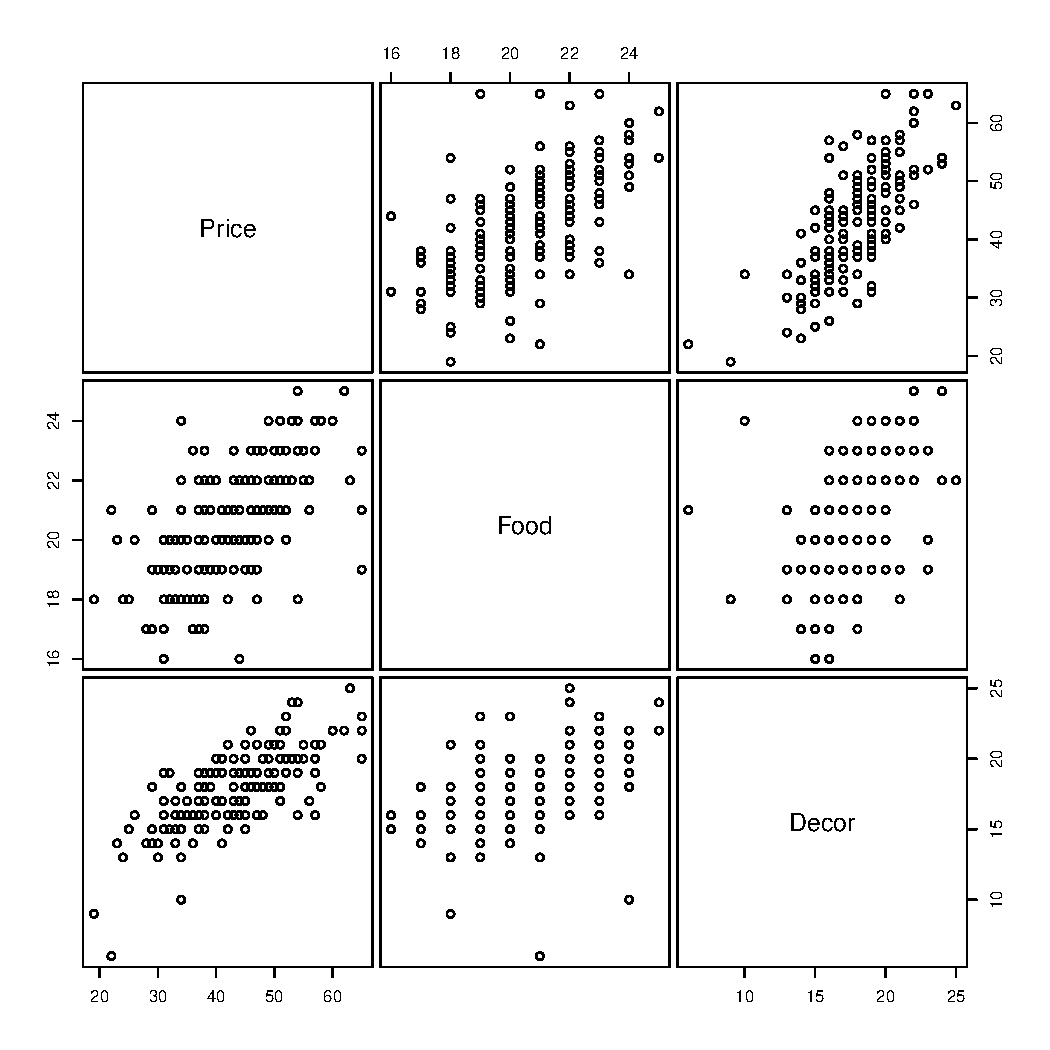
\includegraphics[scale=0.35]{figure/menu_pairs.pdf}
\end{figure}
\end{frame}

%------------------------------------
\begin{frame}
\small
The plot of the standardized residuals versus fitted values shows no discernible trend or nonconstant variance -- the points are randomly scattered around 0. The assumptions of linearity and nonconstant variance appear satisfied.  The QQ plot also indicates that distribution of the standardized residuals are approximately normal, and that there are no extreme outliers.
\begin{figure}
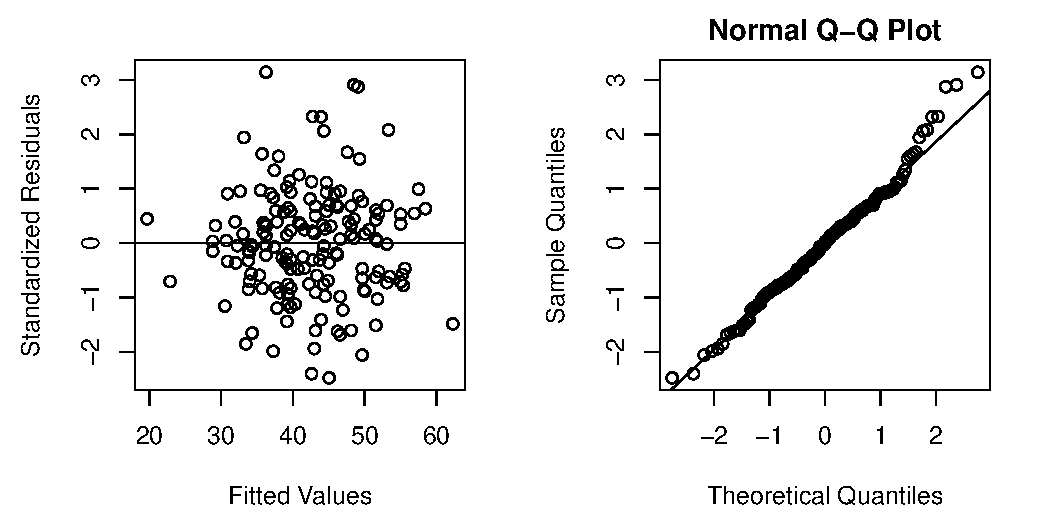
\includegraphics[scale=0.5]{figure/resid_fitted.pdf}
\end{figure}
\end{frame}

%------------------------------------
\begin{frame}
The plots of the residuals versus each predictor also indicate that the MLR assumptions are satisfied.
\begin{figure}
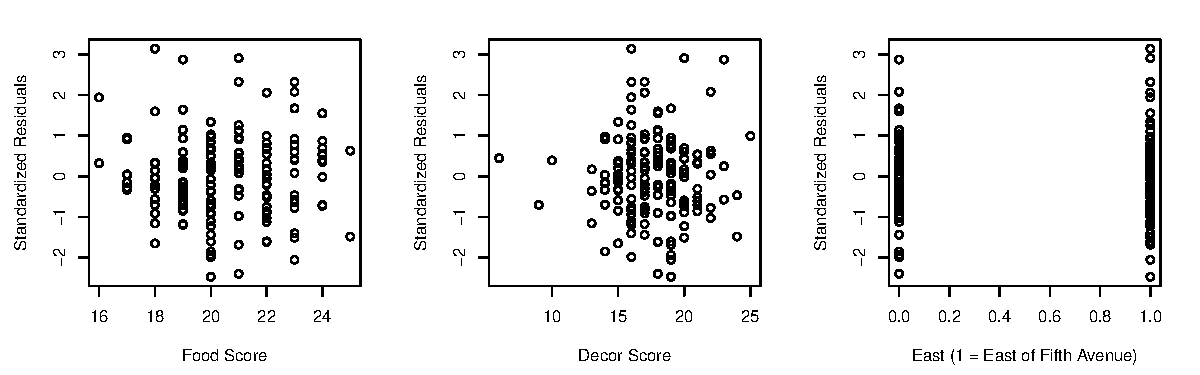
\includegraphics[scale=0.55]{figure/resid_x.pdf}
\end{figure}
\end{frame}

%------------------------------------
\begin{frame}[fragile]
Here is the code for the diagnostic plots:
\small
\begin{verbatim}
# residuals versus fitted and QQ plot
> par(mfrow=c(1,2), mar=c(4.5, 4.5, 2, 2))
> plot(predict(lm2), rstandard(lm2), 
       xlab="Fitted Values", ylab="Standardized Residuals")
> abline(h=0)
> qqnorm(rstandard(lm2))
> qqline(rstandard(lm2))

# residuals versus predictors
> par(mfrow=c(1,3), mar=c(4.5, 4.5, 2, 2))
> plot(nyc$Food, rstandard(lm2), 
       xlab="Food Score", ylab="Standardized Residuals")
> plot(nyc$Decor, rstandard(lm2), 
       xlab="Decor Score", ylab="Standardized Residuals")
> plot(nyc$East, rstandard(lm2), 
       xlab="East (1 = East of Fifth Avenue)", 
       ylab = "Standardized Residuals")
\end{verbatim}
\end{frame}

\begin{frame}[fragile]
\small
\begin{verbatim}
> p <- 3
> n <- nrow(nyc)
> plot(hatvalues(lm2), rstandard(lm2), 
       xlab='Leverage', ylab='Standardized Residuals')
> abline(v = 2*(p+1)/n, lty=2)
\end{verbatim}
\begin{figure}
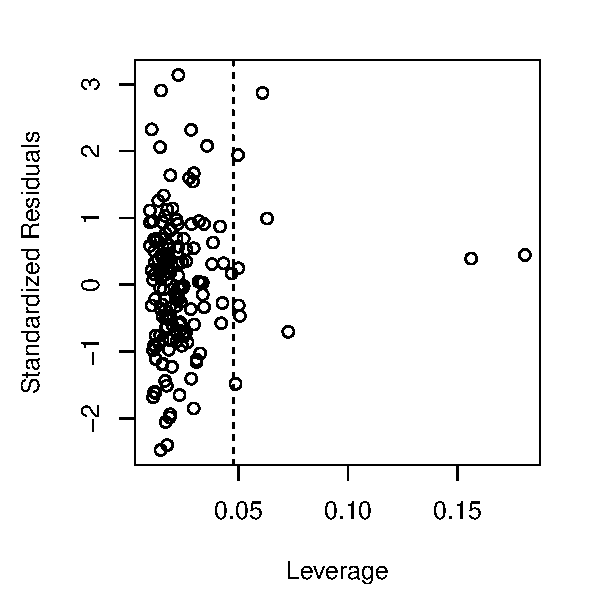
\includegraphics[scale=0.6]{figure/influence1.pdf}
\end{figure}
\end{frame}

\begin{frame}{Your Turn}
\large
Idenitfy the two restaurants with the highest leverages.\\
\end{frame}

\end{document}
